%%%%%%%%%%%%%%%%%%%%%%%%%%%%%%%%%%%%%%%%%%%%%%%%%%%%%%%%%%%%%%%%%%%%%%%%%%%%%%%%%%%%%%%%%%%%%%%%%%%
%%%%%%%%%%%%%%%%%%%%%%%%%%%%%%%%%%%%%%%%%%%%%%%%%%%%%%%%%%%%%%%%%%%%%%%%%%%%%%%%%%%%%%%%%%%%%%%%%%%
%%%%%%%%%%%%%%%%%%%%%%%%%%%%%%%%%%%%%%%%%%%%%%%%%%%%%%%%%%%%%%%%%%%%%%%%%%%%%%%%%%%%%%%%%%%%%%%%%%%
\documentclass[12pt,dvipdfmx]{beamer}
%%%%%%%%%%%%%%%%%%%%%%%%%%%%%%%%%%%%%%%%%%%%%%%%%%%%%%%%%%%%%%%%%%%%%%%%%%%%%%%%%%%%%%%%%%%%%%%%%%%%%%
% pdfの栞・プロパティの字化けを防ぐ
\usepackage{atbegshi}
%\AtBeginShipoutFirst{\special{pdf:tounicode 90ms-RKSJ-UCS2}} %Windows
\AtBeginShipoutFirst{\special{pdf:tounicode EUC-UCS2}} %Linux, Mac
\usepackage{hyperref}
%%%%%%%%%%%%%%%%%%%%%%%%%%%%%%%%%%%%%%%%%%%%%%%%%%%%%%%%%%%%%%%%%%%%%%%%%%%%%%%%%%%%%%%%%%%%%%%%%%%%%%
%%%
%%% テーマの指定、省略時は default になる
%%%

 % フレームの指定、省略可
%%%%%%%%%%%%%%%%%%%%%%%%%%%% THEME
  %\usetheme{AnnArbor}
  %\usetheme{Antibes}
  %\usetheme{Bergen}
  %\usetheme{Berkeley}
  %\usetheme{Berlin}
  \usetheme{Boadilla}
  %\usetheme{boxes}
  %\usetheme{CambridgeUS}
  %\usetheme{Copenhagen}
  %\usetheme{Darmstadt}
  %\usetheme{default}
  %\usetheme{Dresden}
  %\usetheme{Frankfurt}
  %\usetheme{Goettingen}
  %\usetheme{Hannover}
  %\usetheme{Ilmenau}
  %\usetheme{JuanLesPins}
  %\usetheme{Luebeck}
  %\usetheme{Madrid}
  %\usetheme{Malmoe}
  %\usetheme{Marburg}
  %\usetheme{Montpellier}
  %\usetheme{PaloAlto}
  %\usetheme{Pittsburgh}
  %\usetheme{Rochester}
  %\usetheme{Singapore}
  %\usetheme{Szeged}
  %\usetheme{Warsaw}

% 省略可
%%%%%%%%%%%%%%%%%%%%%%%%%%%% COLOR THEME
  %\usecolortheme{albatross}
  %\usecolortheme{beetle}
  %\usecolortheme{crane}
  %\usecolortheme{default}
  %\usecolortheme{dolphin}
  %\usecolortheme{dove}
  %\usecolortheme{fly}
  %\usecolortheme{lily}
  %\usecolortheme{orchid}
  %\usecolortheme{rose}
  %\usecolortheme{seagull}
  %\usecolortheme{seahorse}
  %\usecolortheme{sidebartab}
  %\usecolortheme{structure}
  %\usecolortheme{whale}

% ヘッダ、フッタ、フレーム等を指定、省略可
  %%%%%%%%%%%%%%%%%%%%%%%%%%%% OUTER THEME
  %\useoutertheme{default}
  %\useoutertheme{infolines}
  %\useoutertheme{miniframes}
  %\useoutertheme{shadow}
  %\useoutertheme{sidebar}
  %\useoutertheme{smoothbars}
  %\useoutertheme{smoothtree}
  %\useoutertheme{split}
  %\useoutertheme{tree}

% タイトル、section, itemize/enumerate 環境、
% theorem 環境、図, 参考文献などのスタイルを指定、
% 省略可
  %%%%%%%%%%%%%%%%%%%%%%%%%%%% INNER THEME
  %\useinnertheme{circles}
  %\useinnertheme{default}
  %\useinnertheme{inmargin}
  \useinnertheme{rectangles}
  %\useinnertheme{rounded}


%\usefonttheme{}	% 省略可
%\logo{}		% 省略可

%%%%%%%%%%%%%%%%%%%%%%%%%%%%%%%%%%%%%%%%%%%%%%%%%%%%%%%%%%%%%%%%%%%%%%%%%%%%%%%%%%%%%%%%%%%%%%%%%%%
%%%%%%%%%%%%%%%%%%%%%%%%%%%%%%%%%%%%%%%%%%%%%%%%%%%%%%%%%%%%%%%%%%%%%%%%%%%%%%%%%%%%%%%%%%%%%%%%%%%
%%%%%%%%%%%%%%%%%%%%%%%%%%%%%%%%%%%%%%%%%%%%%%%%%%%%%%%%%%%%%%%%%%%%%%%%%%%%%%%%%%%%%%%%%%%%%%%%%%%
% navi. symbolsは目立たないが,dvipdfmxを使うと機能しないので非表示に
\setbeamertemplate{navigation symbols}{}

% 各種パッケージ
\usepackage{graphicx}
%\usepackage{url,cite}
\usepackage{amsmath}
\usepackage{amsthm} \theoremstyle{definition} %theorem環境が斜体になるので注意
\usepackage{amssymb} % AMS-TeX
\usepackage{setspace}

% \AtBeginSection[] % Do nothing for \section*
% { \begin{frame}<beamer> \frametitle{}
%    \tableofcontents[currentsection,subsectionstyle=hide]
%  \end{frame} } 

%appendixをページカウントしない
\newcommand{\backupbegin}{
   \newcounter{framenumberappendix}
   \setcounter{framenumberappendix}{\value{framenumber}}
}
\newcommand{\backupend}{
   \addtocounter{framenumberappendix}{-\value{framenumber}}
   \addtocounter{framenumber}{\value{framenumberappendix}} 
}

%%%%%%%%%%%%%%%%%%%%%%%%%%%%%%%%%%%%%%%%%%%%%%%%%%%%%%%%%%%%%%%%%%%%%%%%%%%%%%%%%%%%%%%%%%%%%%%%%%%%%%
% 本文・数式フォント
%\usepackage{palatino,mathpazo}
%\usepackage{times,mathptmx}
\usepackage[varg]{txfonts}
%\usepackage[varg]{pxfonts}

% \mathcal(\cal)の扱い
%\DeclareMathAlphabet{\mathcal}{OMS}{cmsy}{m}{n} %computer modern
%\DeclareMathAlphabet{\mathcal}{OMS}{txsy}{m}{n} %txfont
%\usepackage[psamsfonts]{eucal} % euler

% mathptmx時に数式モードのvをtxfontから借りる
% \DeclareSymbolFont{lettersA}{U}{txmia}{m}{it}
% \SetSymbolFont{lettersA}{bold}{U}{txmia}{bx}{it}
% \DeclareFontSubstitution{U}{txmia}{m}{it}
% \DeclareMathSymbol{v}{\mathalpha}{lettersA}{"33} %"


%上線 widebar, Widebar
\usepackage{accents}
\makeatletter
\def\widebar{\accentset{{\cc@style\underline{\mskip11mu}}}}
\makeatother


%%%%%%%%%%%%%%%%%%%%%%%%%%%%%%%%%%%%%%%%%%%%%%%%%%%%%%%%%%%%%%%%%%%%%%%%%%%%%%%%%%%%%%%%%%%%%%%%%%%%%%

% 定理環境
% \newtheorem{theorem}{Theorem}
% \newtheorem{lemma}[theorem]{Lemma}
% \newtheorem{corollary}[theorem]{Corollary}
% \newtheorem{definition}[theorem]{Definition}
% \newtheorem{example}[theorem]{Example}
\newtheorem{proposition}{Proposition}
\newtheorem{remark}{Remark}

%%%%%%%%%%%%%%%%%%%%%%%%%%%%%%%%%%%%%%%%%%%%%%%%%%%%%%%%%%%%%%%%%%%%%%%%%%%%%%%%%%%%%%%%%%%%%%%%%%%%%%
% 各種コマンド定義等
\def\Fig#1{Fig.\@\ref{#1}}
\def\Table#1{Table~\ref{#1}}
\def\Eq#1{Eq.\@(\ref{#1})}
\def\Eqs#1{Eqs.\@(\ref{#1})}
\def\Thm#1{Theorem~\ref{#1}}
\def\Lma#1{Lemma~\ref{#1}}
\def\Sect#1{Section~\ref{#1}}
\def\Rmk#1{Remark~\ref{#1}}
\def\Prop#1{Proposition~\ref{#1}}
\def\Coro#1{Corollary~\ref{#1}}
\def\Def#1{Definition~\@\ref{#1}}
\def\Prob#1{Problem~\@\ref{#1}}
\def\ie{{i.\@e.\@,~}}
\def\eg{{e.\@g.\@,~}}
\def\etal{{et al.}}

% 数式環境用
\def\rank{\mathsf{rank}\, }
\def\dim{\mathsf{dim}\, }
\def\rspace{\mathsf{span}}
\def\supp{\mathsf{supp}}
%\def\vec#1{\mathbf{#1}}
\def\F{\mathbb{F}}
\def\wt{\mathsf{wt}}
\def\c{\mathcal{C}}
\def\dc{\mathcal{C}^{\perp}}
\def\d{\mathcal{D}}
\def\dd{\mathcal{D}^{\perp}}
\def\g{\mathcal{G}}
\def\dg{\mathcal{G}^{\perp}}
\def\p{\mathcal{P}}
% \def\rspace{\mathsf{span}}
\def\supp{\mathsf{supp}}
\def\ker{\mathsf{Ker\ }}

%\def\bari#1{\{\widebar{#1}\}}
\def\bari#1{\,\overline{{\!\{#1\}\!}}\,}
%\def\bari#1{\bar{\{#1\}}}
\def\vecxi{Z_{\bari{i}}}
%\def\vecsxi{\vec{z}_i}
\def\tvector{X}
\def\tpackets{X_1,\dots,X_n}
\def\mvector{S}
\def\mpackets{S_1,\dots,S_l}
\def\rvector{Y}
\def\wvector{W}
\def\cvector{C}
\def\cword{C_{1},\dots,C_{l+n}}
\def\pcword{C_{l+1},\dots,C_{l+n}}
\def\randvector{R}

\def\compmat{\Phi}

%%%%%%%%%%%%%%%%%%%%%%%%%%%%%%%%%%%%%%%%%%%%%%%%%%%%%%%%%%%%%%%%%%%%%%%%%%%%%%%%%%%%%%%%%%%%%%%%%%%
%%%%%%%%%%%%%%%%%%%%%%%%%%%%%%%%%%%%%%%%%%%%%%%%%%%%%%%%%%%%%%%%%%%%%%%%%%%%%%%%%%%%%%%%%%%%%%%%%%%
%%%%%%%%%%%%%%%%%%%%%%%%%%%%%%%%%%%%%%%%%%%%%%%%%%%%%%%%%%%%%%%%%%%%%%%%%%%%%%%%%%%%%%%%%%%%%%%%%%%
%%%
%%%  日本語フォントをゴシックに、数式フォントを太字に変更する
%%%
\renewcommand{\kanjifamilydefault}{\gtdefault}
\renewcommand{\familydefault}{\sfdefault}

\setbeamerfont{title}{size=\large,series=\bfseries}
\setbeamerfont{frametitle}{size=\large,series=\bfseries}
%\setbeamertemplate{frametitle}[default][center]
\usefonttheme{professionalfonts} 

%\mathversion{bold} %数式フォントを太字に

%\def\vec#1{\mbox{\boldmath $#1$}}


%\logo{\includegraphics[width=2cm]{titech_logo.eps}}

%\setbeamertemplate{caption}[numbered]
%%%
%%% 著者など
%%%
\title[E2E Security with JS 03]{JavaScriptによるEnd-to-Endセキュリティ}
\subtitle{第3回 公開鍵暗号はどうやって使えばいいのか? 編\\ \alert{PNGになってんのはPDFに修正しとくこと}}
\author[Jun Kurihara]{栗原 淳}
\institute[]{}
\date[Oct. 17, 2019]{2019年10月17日}

%%%%%%%%%%%%%%%%%%%%%%%%%%%%%%%%%%%%%%%%%%%%%%%%%%%%%%%%%%%%%%%%%%%%%%%%%%%%%%%%%%%%%%%%%%%%%%%%%%%
%%%%%%%%%%%%%%%%%%%%%%%%%%%%%%%%%%%%%%%%%%%%%%%%%%%%%%%%%%%%%%%%%%%%%%%%%%%%%%%%%%%%%%%%%%%%%%%%%%%
%%%%%%%%%%%%%%%%%%%%%%%%%%%%%%%%%%%%%%%%%%%%%%%%%%%%%%%%%%%%%%%%%%%%%%%%%%%%%%%%%%%%%%%%%%%%%%%%%%%
%%%%%%%%%%%%%%%%%%%%%%%%%%%%%%%%%%%%%%%%%%%%%%%%%%%%%%%%%%%%%%%%%%%%%%%%%%%%%%%%%%%%%%%%%%%%%%%%%%%
%%%%%%%%%%%%%%%%%%%%%%%%%%%%%%%%%%%%%%%%%%%%%%%%%%%%%%%%%%%%%%%%%%%%%%%%%%%%%%%%%%%%%%%%%%%%%%%%%%%

\begin{document}

\begin{frame}
\titlepage
\end{frame}

%%%%%%%%%%%%%%%%%%%%%%%%%%%%%%%%%%%%%%%%%%%%%%%%%%%%%%%%%%%%%%%%%%%%%%%%%%%%%%%%%%%%%%%%%%%%%%%%%%%
\section{はじめに}
\begin{frame}
 \centering
 {\Large はじめに}
\end{frame}

\begin{frame}
\frametitle{はじめに}
第1回と第2回では
\begin{itemize}
 \item End-to-End (E2E) セキュリティの原則と必要性
 \item WebサイトでのE2Eセキュリティ実践のため、JavaScriptで暗号(AES)を正しく・安全に利用する方法
\end{itemize}
を勉強した。


\vspace{2ex}

ところで、AES(共通鍵暗号)とは別に、「公開鍵暗号」というのが存在する。
\end{frame}

\begin{frame}
\frametitle{公開鍵暗号って?}

既知だと思うが、まずざっと定義しておく。

\begin{block}{\small 定義: 公開鍵暗号}
\footnotesize
以下のステップで暗号化・復号が行われる暗号方式のこと
\begin{enumerate}
 \item \underline{特殊な数学的条件}を満たす鍵ペア「公開鍵 $\mathit{PK}$ と 秘密鍵 $\mathit{SK}$」を生成
 \item \alert{$\mathit{PK}$は公開、$\mathit{SK}$は秘匿}
 \item データ$D$を$\mathit{PK}$によって暗号化して、暗号化データ$X$を生成
 \item $X$は$\mathit{SK}$によってデータ$D$に復号される。
\end{enumerate}
\end{block}
\end{frame}

\begin{frame}

暗号化・復号の鍵を分けて、暗号化の鍵を公開してしまうことで\alert{パスワードなどの共有が不要}になる。

\begin{center}
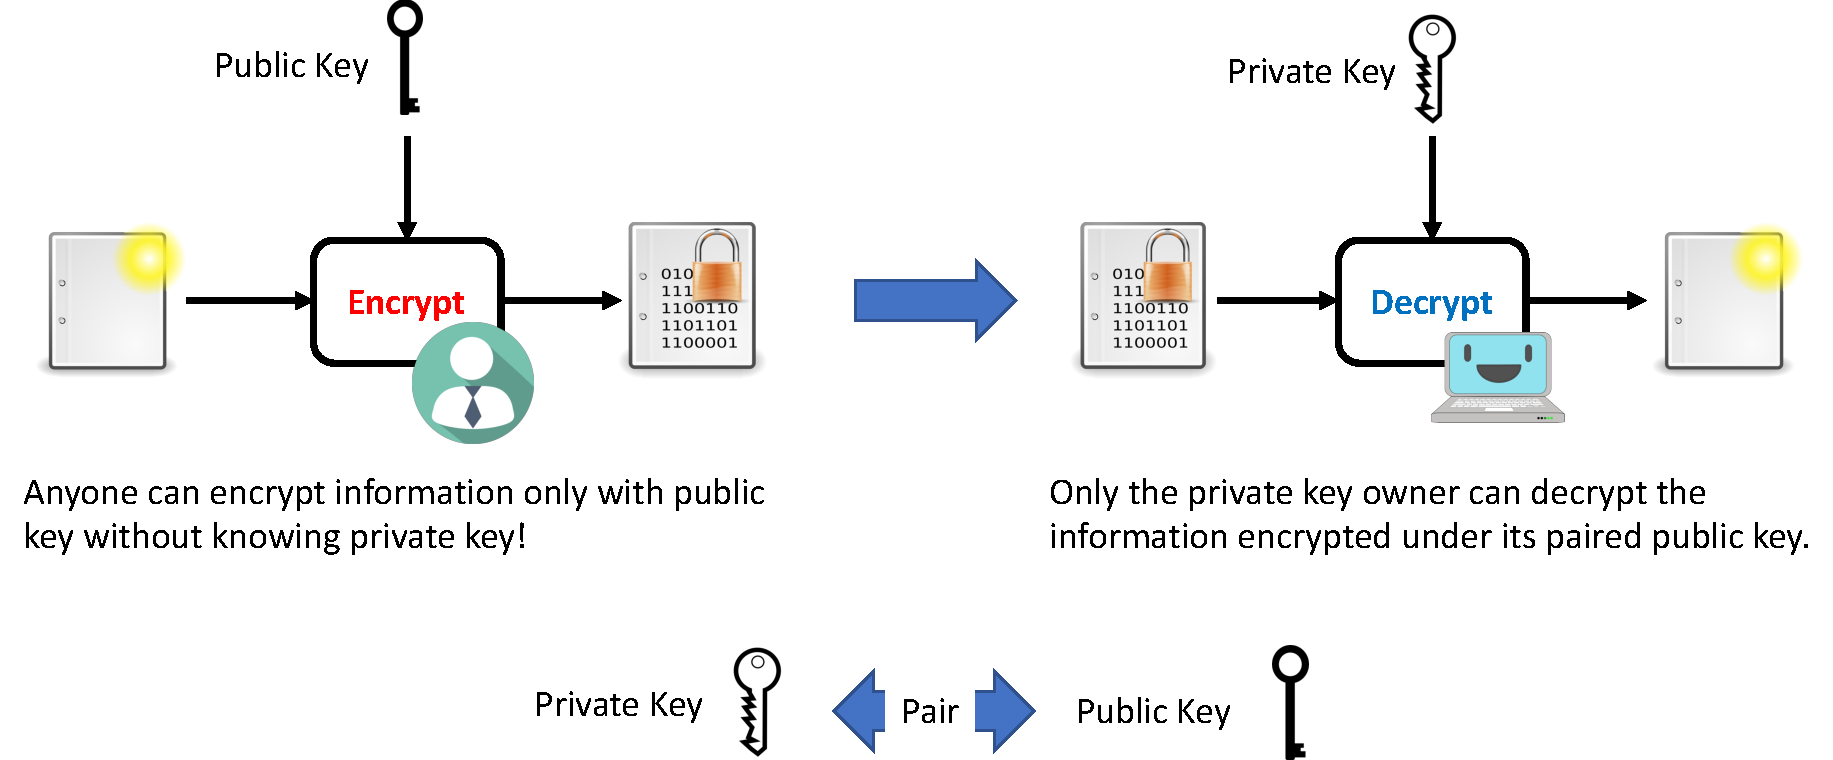
\includegraphics[width=\linewidth]{Figs/pk_cryptosystem.pdf}
\end{center}

\vspace{1ex}

$\Rightarrow$ AESなどにはない、非常に強力な暗号化の概念。現代のセキュリティインフラはこれで成り立っていると言っても過言ではない。
\end{frame}

\begin{frame}
今回は\underline{正しく・安全に}公開鍵暗号を使っていくためのお話。

\begin{block}{\small この講義で最終的に学びたいこと}
\begin{itemize}
\item 公開鍵暗号はどういうものか。AESと比べたpros/cons。
\item RSA暗号と楕円曲線暗号\footnote[frame]{楕円曲線Diffie-Hellmanを取り上げる}の違い。
\item AESと公開鍵暗号を組み合わせてデータを暗号化するために。
\end{itemize}
\end{block}

細かい話もするが、数式は使わない。

「イメージ」と「コードの流れ&その流れの必要性」をつかめるようにする。
\end{frame}


\begin{frame}
\frametitle{この講義の対象と事前準備}
対象:
\begin{itemize}
\item 暗号・セキュリティ技術に興味がある初学者
\item Webに暗号技術を導入したいWeb系のエンジニア
\end{itemize}

\vspace{2ex}

必須ではないが触って楽しむのには必要な事前準備:
\begin{itemize}
\item Bash, Gitが使えるようになっていること
\item Node.js, npm, yarnが使えるようになっていること
\item Google Chrome系ブラウザ and/or Firefoxが利用可能なこと
\end{itemize}
\end{frame}


%%%%%%%%%%%%%%%%%%%%%%%%%%%%%%%%%%%%%%%%%%%%%%%%%%%%%%%%%%%%%%%%%%%%%%%%%%%%%%%%%%%%%%%%%%%%%%%%%%%
\section{公開鍵暗号の使い方 事始め}
\begin{frame}
\centering
{\Large 公開鍵暗号の使い方 事始め}
\end{frame}

\begin{frame}
\frametitle{公開鍵暗号の種類}
\begin{exampleblock}{}
\begin{center}
公開鍵暗号の定義「\underline{特殊な数学的条件}を満たす鍵ペアを生成」\\[0.5ex]
 $\Downarrow$\\[0.5ex]
この「数学的条件」に複数の種類が存在。
\end{center}
\end{exampleblock}

\vspace{2ex}

JavaScriptに限らず、各種環境で利用可能な代表的な公開鍵暗号:
\begin{itemize}
 \item 素因数分解に関する条件\\ → \alert{RSA暗号}
 \item 楕円曲線上の離散対数に関する条件\\ → \alert{楕円曲線暗号(Elliptic Curve Diffie-Hellman; ECDH)}
\end{itemize}
この2つの使い方、注意ポイントを今回は取り上げる。
\end{frame}

\begin{frame}
\frametitle{RSA暗号のさわり}
\begin{block}{RSA Cryptography}
言わずもがな、公開鍵暗号の代表的な手法
\begin{itemize}
 \item 1977年、Rivest-Shamir-Edelmanの3名により発明。2000年に特許期間満了(現在特許フリー)。暗号化以外に「署名」の手法への応用も有名。
 \item RFC 8017 (PKCS\#1 v2.2)、ANSI X9.31、IEEE 1363、CRYPTREC等、各所で標準に採用。
 \item 公開鍵長は1024--4096bitsが標準的に使われている。\footnote[frame]{原理的には無限に伸ばせる。}
 \item 暗号化・署名の際には、元のデータにパディングが必要。\alert{パディング方法によりセキュリティが大きく左右される。}\footnote[frame]{RSA-OAEP(暗号化)、RSA-PSS(署名)が現状ベターな方法。これを話す。}
\end{itemize}
\end{block}

\end{frame}

\begin{frame}
\frametitle{楕円曲線暗号のさわり}
\begin{block}{Elliptic-Curve Cryptography}
楕円曲線という数の世界での「離散対数」を使った方式の総称\footnote[frame]{\scriptsize 普通に離散対数問題を使うより、楕円曲線上でやることで安全性を担保する鍵長が短くなる。}
\begin{itemize}
\item 1985年頃、Victor Miller、Neal Koblitzにより独立に考案。
\item Diffie-Hellman(DH)\footnote[frame]{\scriptsize RFC2631 \url{https://tools.ietf.org/html/rfc2631}}を楕円曲線上で実行するのがECDH、DSA\footnote[frame]{\scriptsize NIST FIPS 186-4 \url{https://nvlpubs.nist.gov/nistpubs/FIPS/NIST.FIPS.186-4.pdf}}を楕円曲線上で実行するのがECDSA。
\item RFC8442、CRYPTREC、IEEE P1363等で標準化。TLSやBitcoinなど多方面で利用。
\item 公開鍵長は256--521bits (Compact form) が標準的に使われている。
\item ECDHは「ECDH-Ephemeral」という方法で実行することで、普通に使うより\alert{安全性が大きく向上}する。\footnote[frame]{\scriptsize Forward Secrecy(第1回のスライド参照)を担保する。}
\end{itemize}
\end{block}
\end{frame}

\begin{frame}
\frametitle{AESと比べた公開鍵暗号のPros/Cons}
\small

何でもかんでも公開鍵暗号、で良さそうな気もしてくるが…

\begin{table}
\centering
\begin{tabular}{|p{0.1\linewidth}||p{0.39\linewidth}|p{0.39\linewidth}|}
\hline
 & \textbf{Pros} & \textbf{Cons}\\
\hline
\hline
\textbf{AES}
& ・安全性を担保する鍵長が短い (128bits〜) & ・パスワードなどの\structure{事前共有が必要} \\
& ・一般的に\alert{高速}・SoCでの最適化も望める\footnote[frame]{Intel AES-NI} & \\
\hline
\textbf{公開鍵暗号}
& ・パスワードなどの秘密情報の\alert{事前共有が不要} & ・安全性を担保する鍵長が長い (RSA: 2048bits〜)\\
& & ・一般的に\structure{非常に遅い・重い}\\
\hline
\end{tabular}
\end{table}

$\Rightarrow$ 使い所を考えて組み合わせて使う、もしくは場合に応じて使い分けないと\structure{実用に耐えないシステム・サービスが出来上がる}。


\end{frame}

\begin{frame}
\frametitle{安全性を担保する鍵長が大きく違うのはどういうこと?}

AESと比べたRSA・楕円曲線暗号の鍵のビット長比較\footnote[frame]{\scriptsize Recommendation for Key Management, Special Publication 800-57 Part 1 Rev. 4, NIST, 01/2016. \url{https://csrc.nist.gov/publications/detail/sp/800-57-part-1/rev-4/final}}。\alert{横1行がだいたい同じくらいの安全性}と言われる。
\begin{table}
\centering
\begin{tabular}{|c||c|c|}
\hline
\textbf{AES} & \textbf{RSA} & \textbf{楕円曲線}\\
\hline
\hline
128 & 3072 & 256--383\\
\hline
192 & 7680 & 384--511\\
\hline
256 & 15360 & 512--\\
\hline
\end{tabular}
\end{table}

\begin{block}{}
AESに比べて、\alert{楕円曲線で倍、RSAに至っては24倍以上}の鍵長を使わないと、同じくらいの安全性を担保できない。
\end{block}

※ \structure{鍵長は長ければ長いほど処理がどんどん重く・遅くなっていく…}

\end{frame}
\begin{frame}
 
「AES-128が、RSA-3072と同じくらい」というイメージは、以下のように説明できる。
\begin{itemize}
 \item AES: 数値$=0,1,\dots,2^{128}-1$のうち、どれか1つが鍵。
 \item RSA: \alert{特殊な条件を満たす数 = 素数2個の積(合成数)}を選んで、公開・秘密鍵を求める。
\end{itemize}

\begin{center}
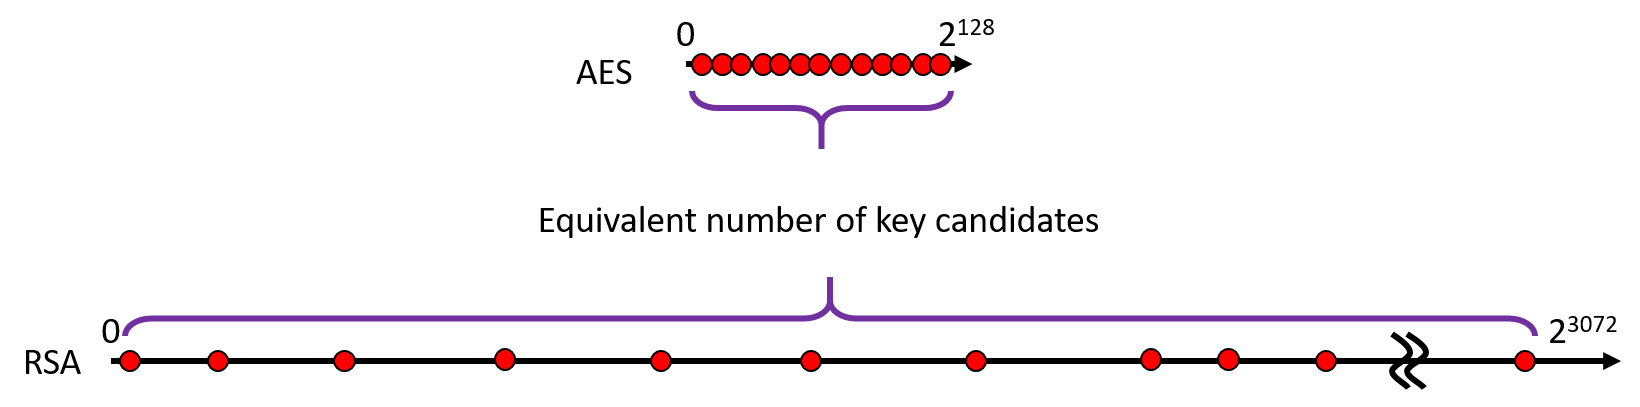
\includegraphics[width=\linewidth]{Figs/key-length-image.png} % todo
\end{center}

総当たりした時に\alert{「当たる」確率を揃えるには、RSAはその分巨大な数まで候補にしないとならない}。
\end{frame}

%%%%%%%%%%%%%%%%%%%%%%%%%%%%%%%%%%%%%%%%%%%%%%%%%%%%%%%%%%%%%%%%%%%%%%%%%%%%%%%%%%%%%%%%%%%%%%%%%%%
\section{今回のサンプル}
\begin{frame}
\centering
{\Large サンプルコードの準備}
\end{frame}

\begin{frame}
\frametitle{準備}
\small
細かく暗号化の説明を聞きつつ、手を動かすため、まず環境準備。

\alert{今回は、JavaScript (Node.js) を使って手元で公開鍵暗号化・復号。}

\begin{center}
 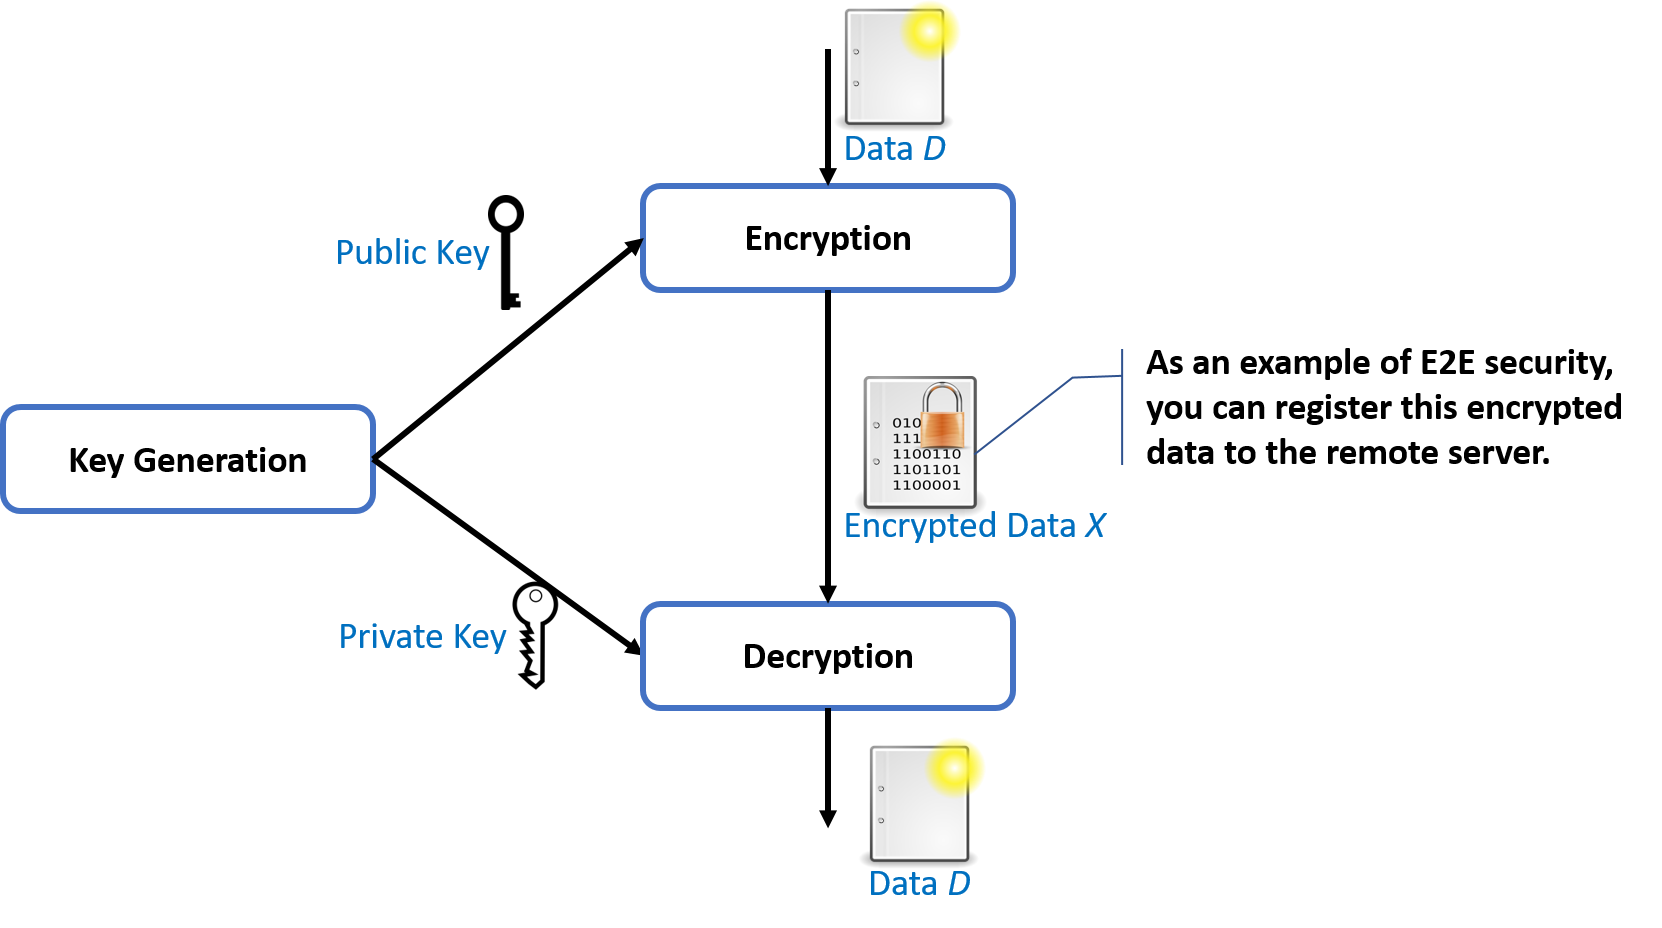
\includegraphics[width=0.8\linewidth]{Figs/pk-flow.png}%todo
\end{center}

前回・前々回使った「リモートサーバに登録する」というところは、簡略化のため端折ってる。興味があれば、前回のコードを公開鍵暗号に拡張して、E2Eセキュリティしてみよう!
\end{frame}

\begin{frame}
\frametitle{環境}
以下の環境が前提:
\begin{itemize}
 \item Node.js ($>$ v10)がインストール済。yarnが使えること。 \footnote[frame]{インストールコマンド: \texttt{npm i -g yarn}}
 \item ブラウザとして、Google Chrome (系ブラウザ)、もしくはFirefoxがインストール済み
 \item Visual Studio Code や WebStorm などの統合開発環境がセットアップ済みだとなお良い。
\end{itemize}
\end{frame}

\begin{frame}
\frametitle{JavaScriptプロジェクトの準備}
\begin{itemize}
\item プロジェクトのGitHubリポジトリ\footnote[frame]{\url{https://github.com/zettant/e2e-security-03}}をClone\\
\begin{exampleblock}{}
\footnotesize
\$ \texttt{git clone https://github.com/zettant/e2e-security-03}\\
\$ \texttt{cd e2e-security-03/sample}
\end{exampleblock}
\item 依存パッケージのインストール
\begin{exampleblock}{}
\$ \texttt{yarn install}
\end{exampleblock}
\item ライブラリのビルド
\begin{exampleblock}{}
\$ \texttt{yarn build}
\end{exampleblock}
\end{itemize}
\end{frame}

%%%%%%%%%%%%%%%%%%%%%%%%%%%%%%%%%%%%%%%%%%%%%%%%%%%%%%%%%%%%%%%%%%%%%%%%%%%%%%%%%%%%%%%%%%%%%%%%%%%
\section{RSA暗号を使ってみよう}
\begin{frame}
\centering
{\Large RSA暗号を使ってみよう}
\end{frame}

\begin{frame}
\frametitle{RSA暗号を使うためのお作法}
\begin{block}{\small RSA暗号化の制限}
\alert{データ$D$と、公開鍵$PK$とが、同じビット長でなければならない}
\end{block}
$\Rightarrow$ RSA暗号化の前には、まず\underline{元データへのパディング}\footnote[frame]{\scriptsize 長いデータの場合は切断…}が必要。

\begin{center}
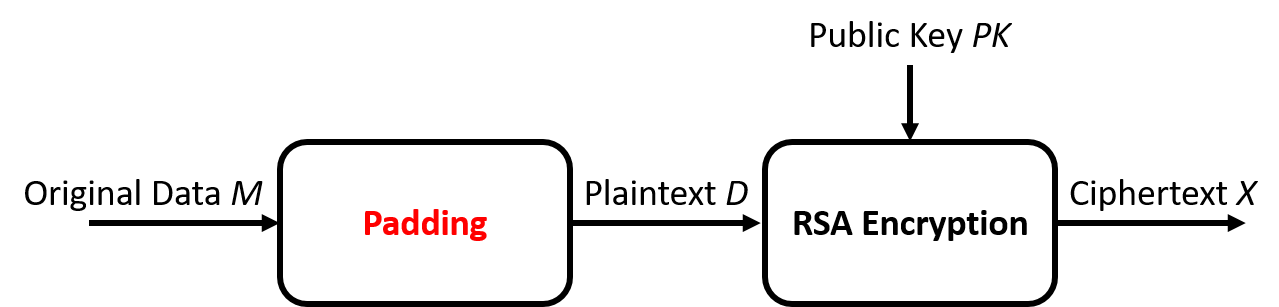
\includegraphics[width=0.9\linewidth]{Figs/rsa-padding.png}\\%todo
\end{center}
\vspace{2ex}

\alert{RSA暗号化には、前処理としてのパディングの選択が最重要のお作法。}
\end{frame}

\begin{frame}

RSA向けに主として2種類のパディング方法が知られている。\footnote[frame]{\scriptsize 共にPKCS\#1 (RFC8017) で標準化。\url{https://tools.ietf.org/html/rfc8017}}

\begin{itemize}
 \item PKCS\#1-v1.5 Padding
 \item Optimal Asymmetric Encryption Padding (OAEP)
\end{itemize}

\end{frame}


\begin{frame}

\begin{block}{\small PKCS\#1-v1.5 Padding}
\small
\begin{itemize}
 \item RSA暗号化と組み合わせると、RSAES-PKCS1-v1\_5。
 \item 元データ$M$に、公開鍵長まで以下のようなパディングを付与。
\begin{align*}
 D = \mathtt{0x00}\ ||\ \mathtt{0x02}\ ||\ \texttt{RandomSequence}\ ||\ \mathtt{0x00}\ ||\ M
\end{align*}
 \item 暗号化データを任意に改変でき、復号者に復号成功・失敗を確認させられる時、\alert{元データを復号される脆弱性}が知られている。\footnote[frame]{\scriptsize 1998年のBleinchenbacher's Attack。 2018年、現代のInternetでも未対策ホスト・サービスが大量なことが発表されている(ROBOT Attack)。}
 \item PKCS\#1 v2.2 (RFC8017) で「後方互換性のため以外では使用するな」と明示的に記載。CRYPTRECにおいても推奨暗号方式リストからドロップ。\footnote[frame]{\scriptsize \url{https://www.cryptrec.go.jp/method.html}}
\end{itemize}
\end{block}

\begin{center}
 {\Large \alert{基本的に使うな}}
\end{center}
\end{frame}

\begin{frame}

\begin{block}{\small Optimal Asymmetric Encryption Padding (OAEP) \footnote[frame]{\scriptsize M. Bellare and P. Rogaway, ``Optimal Asymmetric Encryption,'' in Proc. EUROCRYPTO 1994, pp.~92--111, LNCS 950, 1994.}}
\small
\begin{itemize}
 \item RSA暗号化と組み合わせて、RSA-OAEP、もしくはRSAES (RSA Encryption Scheme) - OAEPと呼ぶ。
 \item 元データ$M$とランダムシードに対して、All or Nothing Transform (AONT)を実行し、$D$を公開鍵ビット長まで膨らませる。
\begin{align*}
 D = \textsf{AONT}(M, \texttt{RandomSeed})
\end{align*}
 \item PKCS\#1-v1.5 Paddingの脆弱性は潰されている。実用の上ですぐに致命的な脆弱性は知られていない。PKCS\#1 v2.2 (RFC8017) では、\alert{新規アプリはOAEPを利用すること}と明記。
\end{itemize}
\end{block}

\begin{center}
 {\Large \alert{今はRSAならOAEP使っとけば間違いない}}
\end{center}
\end{frame}

\begin{frame}
\frametitle{参考: OAEPのイメージ図}
\begin{center}
 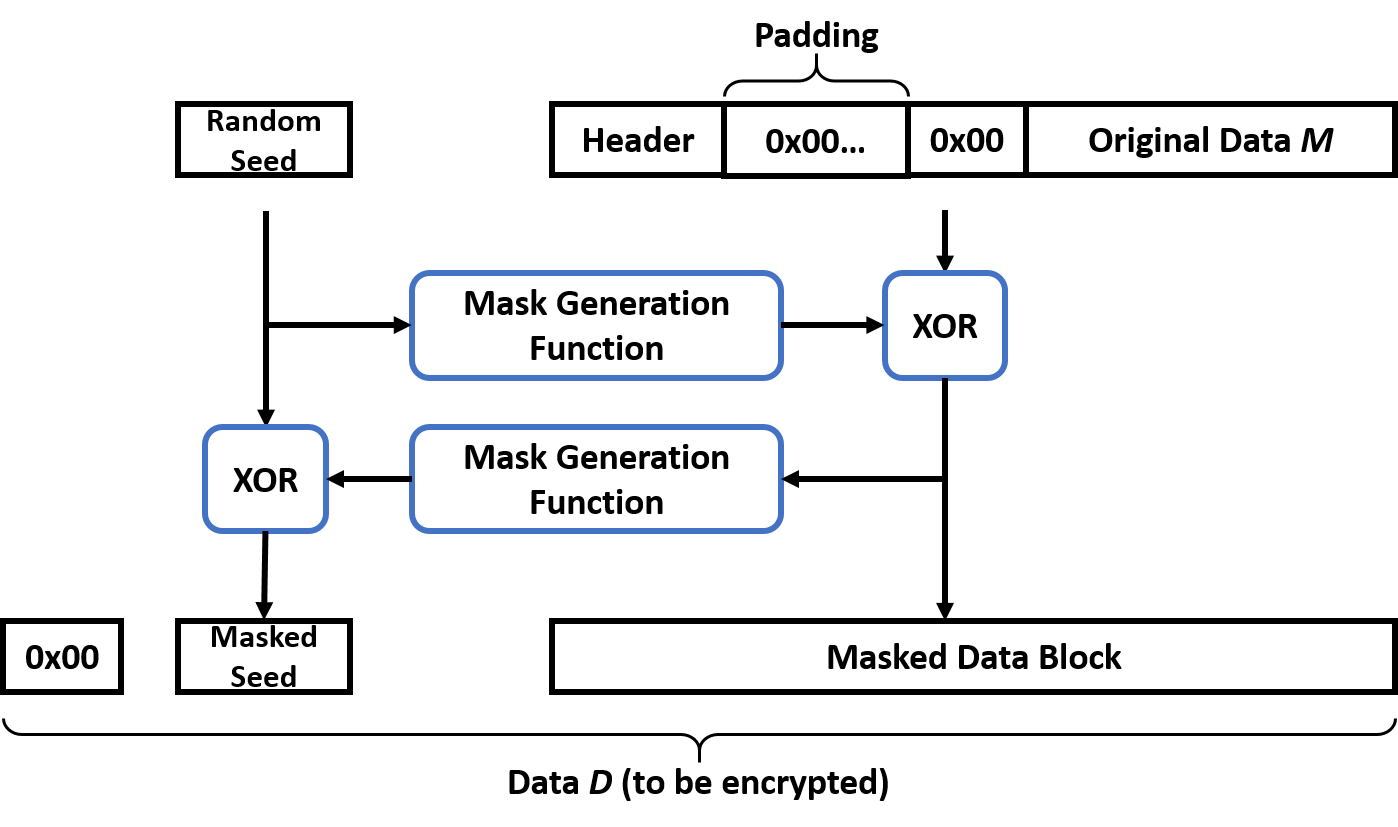
\includegraphics[width=\linewidth]{Figs/oaep.png}
\end{center}
逆変換はMasked Seed, Masked Data Blockが両方揃えば可能。
\end{frame}


\begin{frame}
\frametitle{JavaScriptでRSA-OAEP暗号化をしてみよう}
RSAES-OAEPは、WebCrypto API(ブラウザ)でも、Node.js Cryptoでもネイティブサポートされている。\footnote[frame]{\scriptsize RSAES-PKCS1-v1\_5もサポートされている。}

\end{frame}

\begin{frame}
\end{frame}


%%%%%%%%%%%%%%%%%%%%%%%%%%%%%%%%%%%%%%%%%%%%%%%%%%%%%%%%%%%%%%%%%%%%%%%%%%%%%%%%%%%%%%%%%%%%%%%%%%%
\section{楕円曲線暗号(ECDH)を使ってみよう}
\begin{frame}
\centering
{\Large 楕円曲線暗号(ECDH)を使ってみよう}
\end{frame}

\begin{frame}
\frametitle{楕円曲線暗号を使うためのお作法 その1}

今までECDHを公開鍵暗号って呼んでいてすみませんでした…

\begin{block}{\small Elliptic-Curve Diffie-Hellman (ECDH)}
ECDH自身は、データの暗号化ではなく、公開鍵・秘密鍵を使って\alert{送受信者間で秘密裏にランダムビット列を共有するための方法}。
\end{block}

$\Rightarrow$ 共有したランダムビット列を鍵(の種)として用いて、AESとかでデータを暗号化。

\begin{center}
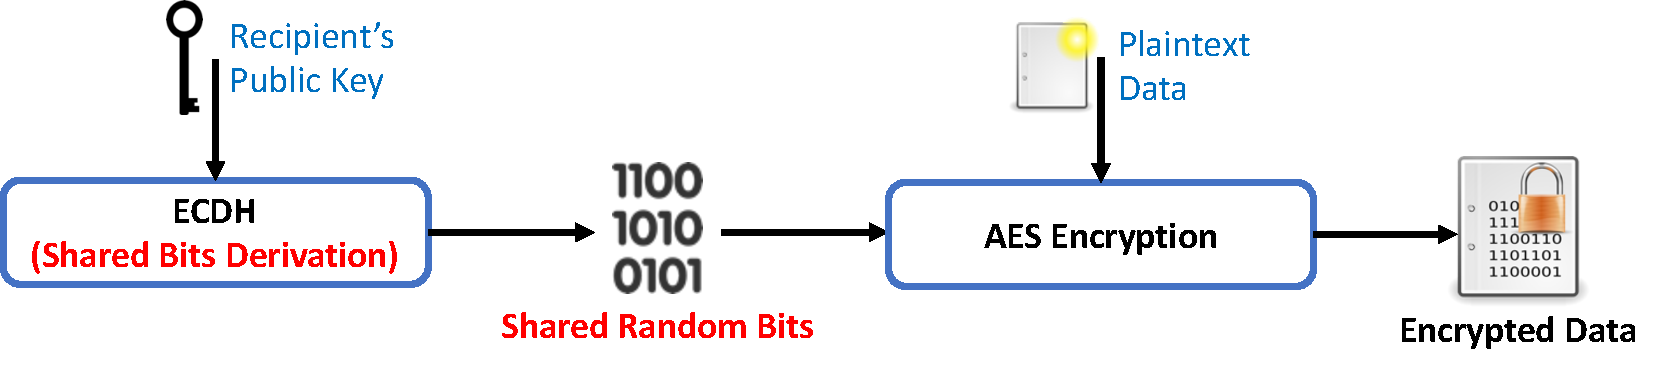
\includegraphics[width=\linewidth]{Figs/ecdh-flow01.pdf}

この流れ全体で「公開鍵暗号」の体を為す。
\end{center}

\end{frame}


\begin{frame}
というわけで、まずはこの「共有ランダムビット列」の導出の話。
\begin{block}{\small ECDHの特徴}
2つの公開鍵・秘密鍵ペア: \alert{$(\mathit{PK_1}, \mathit{SK}_1)$}と\textcolor{blue}{$(\mathit{PK_2}, \mathit{SK}_2)$}で、
\begin{align*}
\mathtt{SharedRandomBits} &= \mathsf{ECDH}(
\text{\textcolor{red}{$\mathit{PK}_1$}},
\text{\textcolor{blue}{$\mathit{SK}_2$}}
)\\
& = \mathsf{ECDH}(
\text{\textcolor{blue}{$\mathit{PK}_2$}},
\text{\textcolor{red}{$\mathit{SK}_1$}}
).
\end{align*}
すなわちECDHでは、\alert{鍵ペアを持っているもの同士なら、相手の公開鍵から共有ビット列が導出可能}。
\end{block}

共有ビット列の長さは、公開鍵長 (Compact form) と一緒。
\end{frame}

\begin{frame}
確認してみよう。
\end{frame}

\begin{frame}
\frametitle{楕円曲線暗号を使うためのお作法 その2}
前回の「AESを使うために」で学んだことの復習。

$\Rightarrow$ 共有ビット列から\alert{正しく・安全に鍵を導出する}こと。\\

\vspace{2ex}

鍵導出関数の利用:
\begin{itemize}
 \item HKDF (RFC5869)
 \item Concat KDF (RFC8039)\footnote[frame]{\scriptsize JOSE向けに標準化された鍵導出関数 \url{https://tools.ietf.org/html/rfc8037}}
 \item etc....
\end{itemize}
$\Rightarrow$ 鍵のランダム具合の向上、鍵の総当たりの困難化。

\end{frame}

\begin{frame}
鍵導出関数を使ってHKDF $\rightarrow$ AES暗号化をしてみよう。
\end{frame}


\section{より実用的な公開鍵暗号の運用}
\begin{frame}
\centering
{\Large より実用的な公開鍵暗号の運用}
\end{frame}

\begin{frame}
\frametitle{公開鍵暗号による、AES暗号鍵のカプセル化}
\begin{block}{\small Hybrid Encryption (ハイブリッド暗号化)}
\end{block}

$\Rightarrow$ 鍵だけを公開鍵暗号、データ自体はAESで暗号化することで、\alert{暗号化データ部分の使い回し}を促進。

\end{frame}

\begin{frame}
Msgpackを使って「複数人宛のデータ暗号化」を試してみよう。 
\end{frame}

\begin{frame}
\frametitle{Perfect Forward Secrecy}
より安全な暗号化のために。

\begin{block}{\small (Perfect) Forward Secrecy}
長期的に保存されているマスター秘密鍵の漏洩や、一部の暗号化データがクラックされたとしても、\alert{それ以外の過去に暗号化されたデータは復号されてしまうことはない}という概念。
\end{block}

\begin{center}
$\Downarrow$\\[1ex]

ハイブリッド暗号化の際、公開鍵・秘密鍵を使い捨てる\alert{Ephemeral Scheme}の利用
\end{center}

\end{frame}

\begin{frame}
 Ephemeral Schemeのイメージ
\end{frame}

\begin{frame}
ECDHを使った暗号化では、Ephemeral Schemeを使うのが推奨される\footnote[frame]{\scriptsize  RSA暗号を使った場合のEphemeral Schemeを標準の手法は知る限りない…単純に巨大な公開鍵を送るコストが高いことと、RSA-4096でAES-256の鍵を暗号化するなど、無駄の多さが理由か?}。


\begin{block}{\small ECDH-Ephemeral (ECDHE)\footnote[frame]{\scriptsize TLSで利用されるスキームだと思って良い \url{https://tools.ietf.org/html/rfc8422}}}
\begin{itemize}
 \item 送信先の相手を問わず、毎回違う共有ビット列が生成される。

$\Rightarrow$ 「今使った」共有ビット列や秘密鍵が盗まれても過去のデータは解読不能。

$\Rightarrow$ \alert{Forward secrecyが担保可能}。
 \item 毎度毎度、まずEphemeral公開鍵を送らなければならず、通信コストは高い。
\end{itemize}
\end{block}

\end{frame}


\begin{frame}
 
\end{frame}

\begin{frame}
 
\end{frame}


%%%%%%%%%%%%%%%%%%%%%%%%%%%%%%%%%%%%%%%%%%%%%%%%%%%%%%%%%%%%%%%%%%%%%%%%%%%%%%%%%%%%%%%%%%%%%%%%%%%
\section{まとめ}
\begin{frame}
 \centering
 {\Large まとめ}
\end{frame}

\begin{frame}
\frametitle{まとめ}
お疲れ様でした。

\begin{itemize}
\item 公開鍵暗号化の際のお作法を学んだ。
\begin{itemize}
 \item RSA: パディングには\alert{OAEPを使う(RSAES-OAEP)}。
 \item ECDH: 導出した共有ビット列は\alert{鍵導出関数を通してから}AESの鍵として利用する。
\end{itemize}
\item より実用的な公開鍵暗号化の運用について触れた。
\begin{itemize}
 \item \structure{ハイブリッド暗号化}: 複数人向け、量的に効率的な暗号化。
 \item \structure{Ephemeral Scheme}: Perfect Forward Secrecyを担保して万一の鍵漏洩に備える。
\end{itemize}
\item 上記について、JavaScriptのコードを実行/中身を覗いてみた。
\end{itemize}
\end{frame}

\begin{frame}
 以下バックアップ
\end{frame}
\begin{frame}
直接Concat KDFを暗号化の鍵にするか、
あるいはConcat KDFの結果をAESKWの鍵としてContent Encryption Keyを暗号化するのに使う。

\end{frame}

\begin{frame}
\frametitle{ECDH Ephemeral (ECDHE)}
\begin{center}
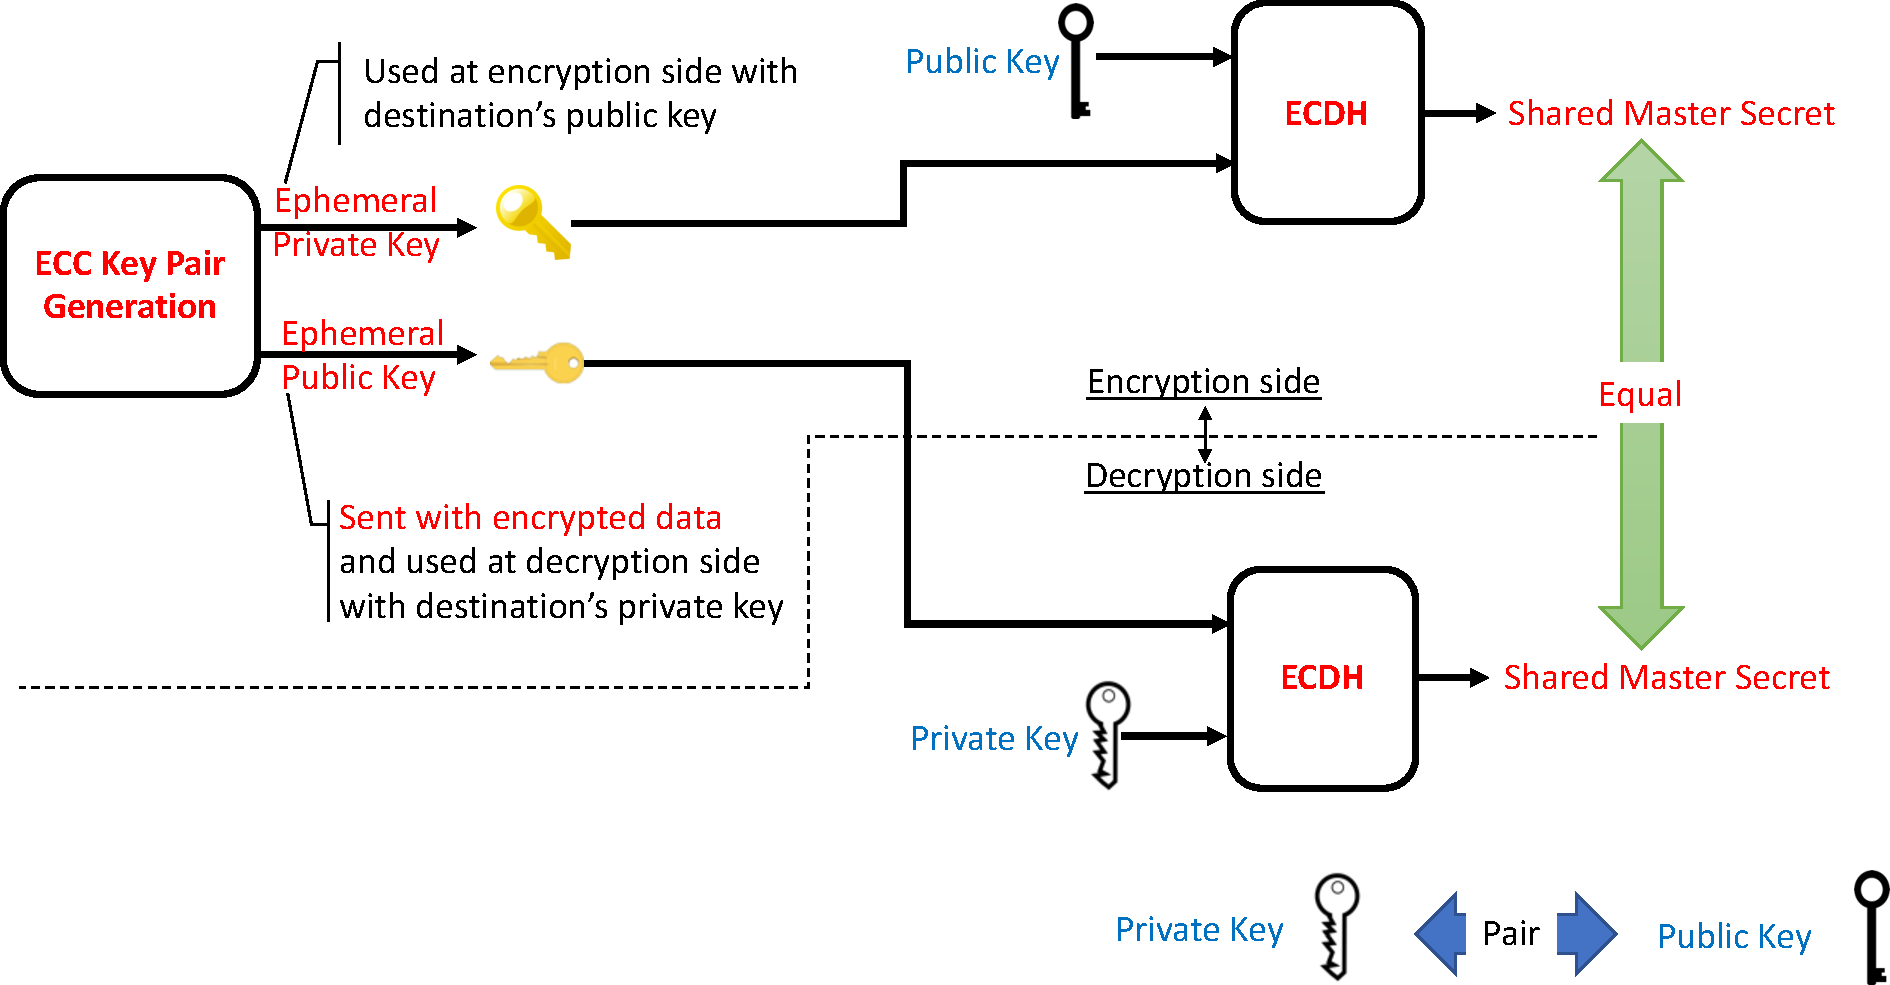
\includegraphics[width=\linewidth]{Figs/ecdh01.pdf}
\end{center}
\end{frame}

\begin{frame}
\begin{center}
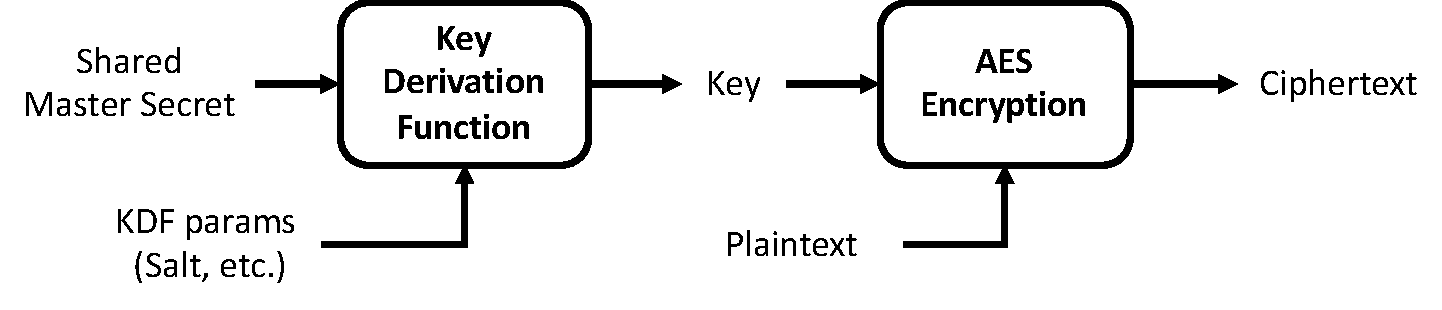
\includegraphics[width=\linewidth]{Figs/ecdh02.pdf}
\end{center}
\end{frame}


\begin{frame}
\begin{center}
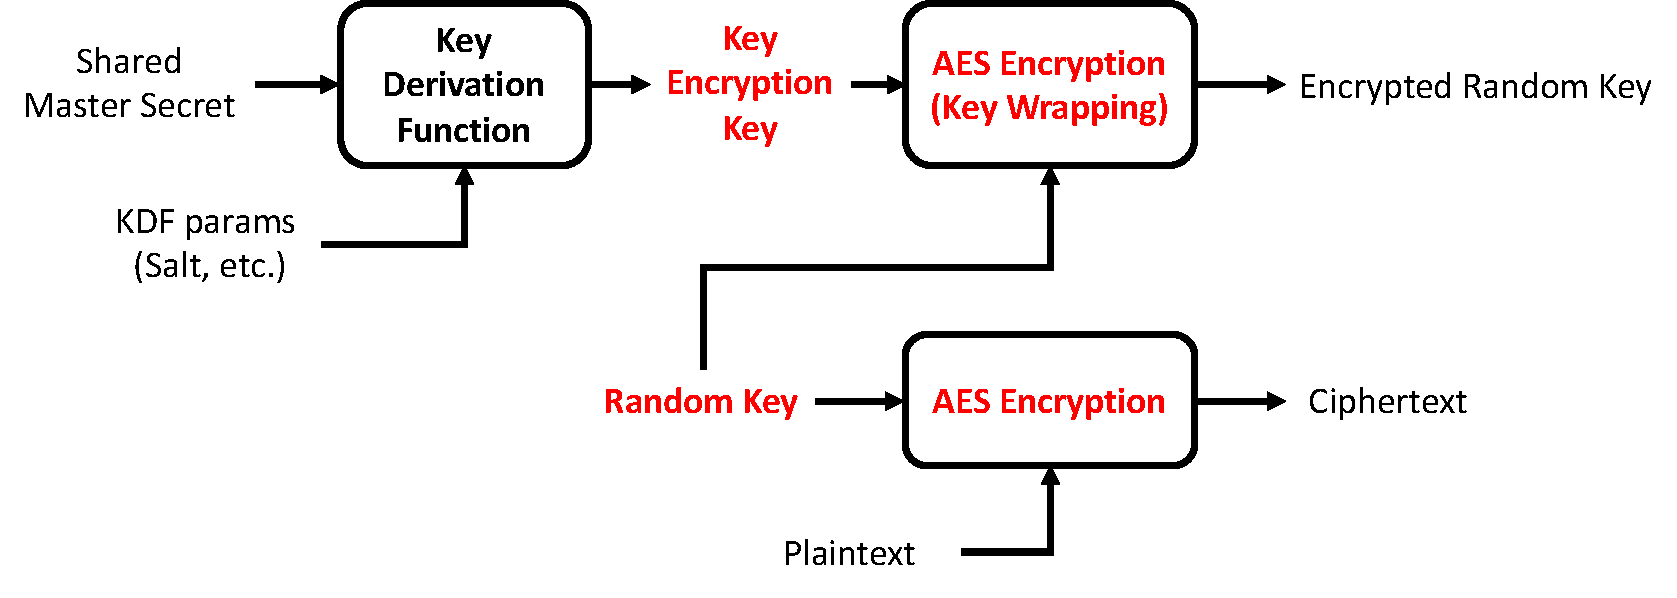
\includegraphics[width=\linewidth]{Figs/aeskw.pdf}
\end{center}
\end{frame}

% \begin{frame}
% 次回以降…リクエスト次第ですが、
% \begin{itemize}
% \item 「情報が改ざんされてない」ことを保証するために(電子署名とMAC)
% \item RFCとアルゴリズム・フォーマット
% \end{itemize}
% などを予定。
% \end{frame}


%%%%%%%%%%%%%%%%%%%%%%%%%%%%%%%%%%%%%%%%%%%%%%%%%%%%%%%%%%%%%%%%%%%%%%%%%%%%%%%%%%%%%%%%%%%%%%%%%%%

% \backupbegin
% \section{Backup}

% \begin{frame}
 
% \end{frame}

% \begin{frame}
%  \begin{enumerate}
%   \item 今回は共通鍵暗号
%   \item 公開鍵暗号\& Hybrid Encryption
%   \item ハッシュ・署名とHMAC
%  \item 超マニアック講座:RFCとアルゴリズム・フォーマット
%  \end{enumerate}
% \end{frame}

% \begin{frame}
% \frametitle{Appendix}
% This page is not counted.
% \end{frame}
% \backupend
\end{document}
%%%%%%%%%%%%%%%%%%%%%%%%%%%%%%%%%%%%%%%%%%%%%%%%%%%%%%%%%%%%%%%%%%%%%%%%%%%%%%%%%%%%%%%%%%%%%%%%%%%
%%%%%%%%%%%%%%%%%%%%%%%%%%%%%%%%%%%%%%%%%%%%%%%%%%%%%%%%%%%%%%%%%%%%%%%%%%%%%%%%%%%%%%%%%%%%%%%%%%%
%%%%%%%%%%%%%%%%%%%%%%%%%%%%%%%%%%%%%%%%%%%%%%%%%%%%%%%%%%%%%%%%%%%%%%%%%%%%%%%%%%%%%%%%%%%%%%%%%%%
%%%%%%%%%%%%%%%%%%%%%%%%%%%%%%%%%%%%%%%%%%%%%%%%%%%%%%%%%%%%%%%%%%%%%%%%%%%%%%%%%%%%%%%%%%%%%%%%%%%
%%%%%%%%%%%%%%%%%%%%%%%%%%%%%%%%%%%%%%%%%%%%%%%%%%%%%%%%%%%%%%%%%%%%%%%%%%%%%%%%%%%%%%%%%%%%%%%%%%%
%%%%%%%%%%%%%%%%%%%%%%%%%%%%%%%%%%%%%%%%%%%%%%%%%%%%%%%%%%%%%%%%%%%%%%%%%%%%%%%%%%%%%%%%%%%%%%%%%%%
